\subsection{Apparato sperimentale}\label{subsec:apparato-sperimentale}
  L’apparato sperimentale è riportato in Fig.\ref{fig:apparato-strumentale}.
  Un prisma(e) di vetro di indice di rifrazione $n_2$ sconosciuto, montato su un servomotore \emph{SM-S2309S}\footnote{http://descargas.cetronic.es/microservo.pdf},
  è posizionato al centro di una guida circolare graduata(d).
  Un laser(a) a luce rossa e due filtri polaroid(b, c) sono
  allineati con il prisma. Un sensore di intensità luminosa(f) \emph{TEMT6000}\footnote{https://www.sparkfun.com/datasheets/Sensors/Imaging/TEMT6000.pdf},
  collegato ad un microcontrollore(g) \emph{Arduino Uno (ATmega328)}\footnote{http://store.arduino.cc/products/arduino-uno-rev3}%
  \footnote{Da qui in avanti, si userà il nome abbreviato \emph{Arduino} al posto di \emph{Arduino Uno} per riferirsi al microcontrollore.},
  è libero di ruotare lungo la guida.
  Il circuito che collega \emph{Arduino} e sensore è schematizzato in Fig.\ref{fig:diagramma-circuito}.
  %
  Il servomotore permette di ruotare il prisma con una risoluzione angolare di ${1.0^\circ \pm 0.5^\circ}$.
  L'apparato Arduino-sensore fornisce una misura dell'intensità luminosa presente
  sulla superficie del sensore nell'intervallo $I = [0, 1000]$ unità arbitrarie,
  con un'incertezza sistematica massima di $0.8\%$ (si rimanda a Sez.\ref{subsec:calcolo-incertezza-strumentale}
  per la dimostrazione di come è stato ottenuto questo valore).
%
  \begin{figure}[h]
    \centering
    \begin{subfigure}{.47\textwidth}
      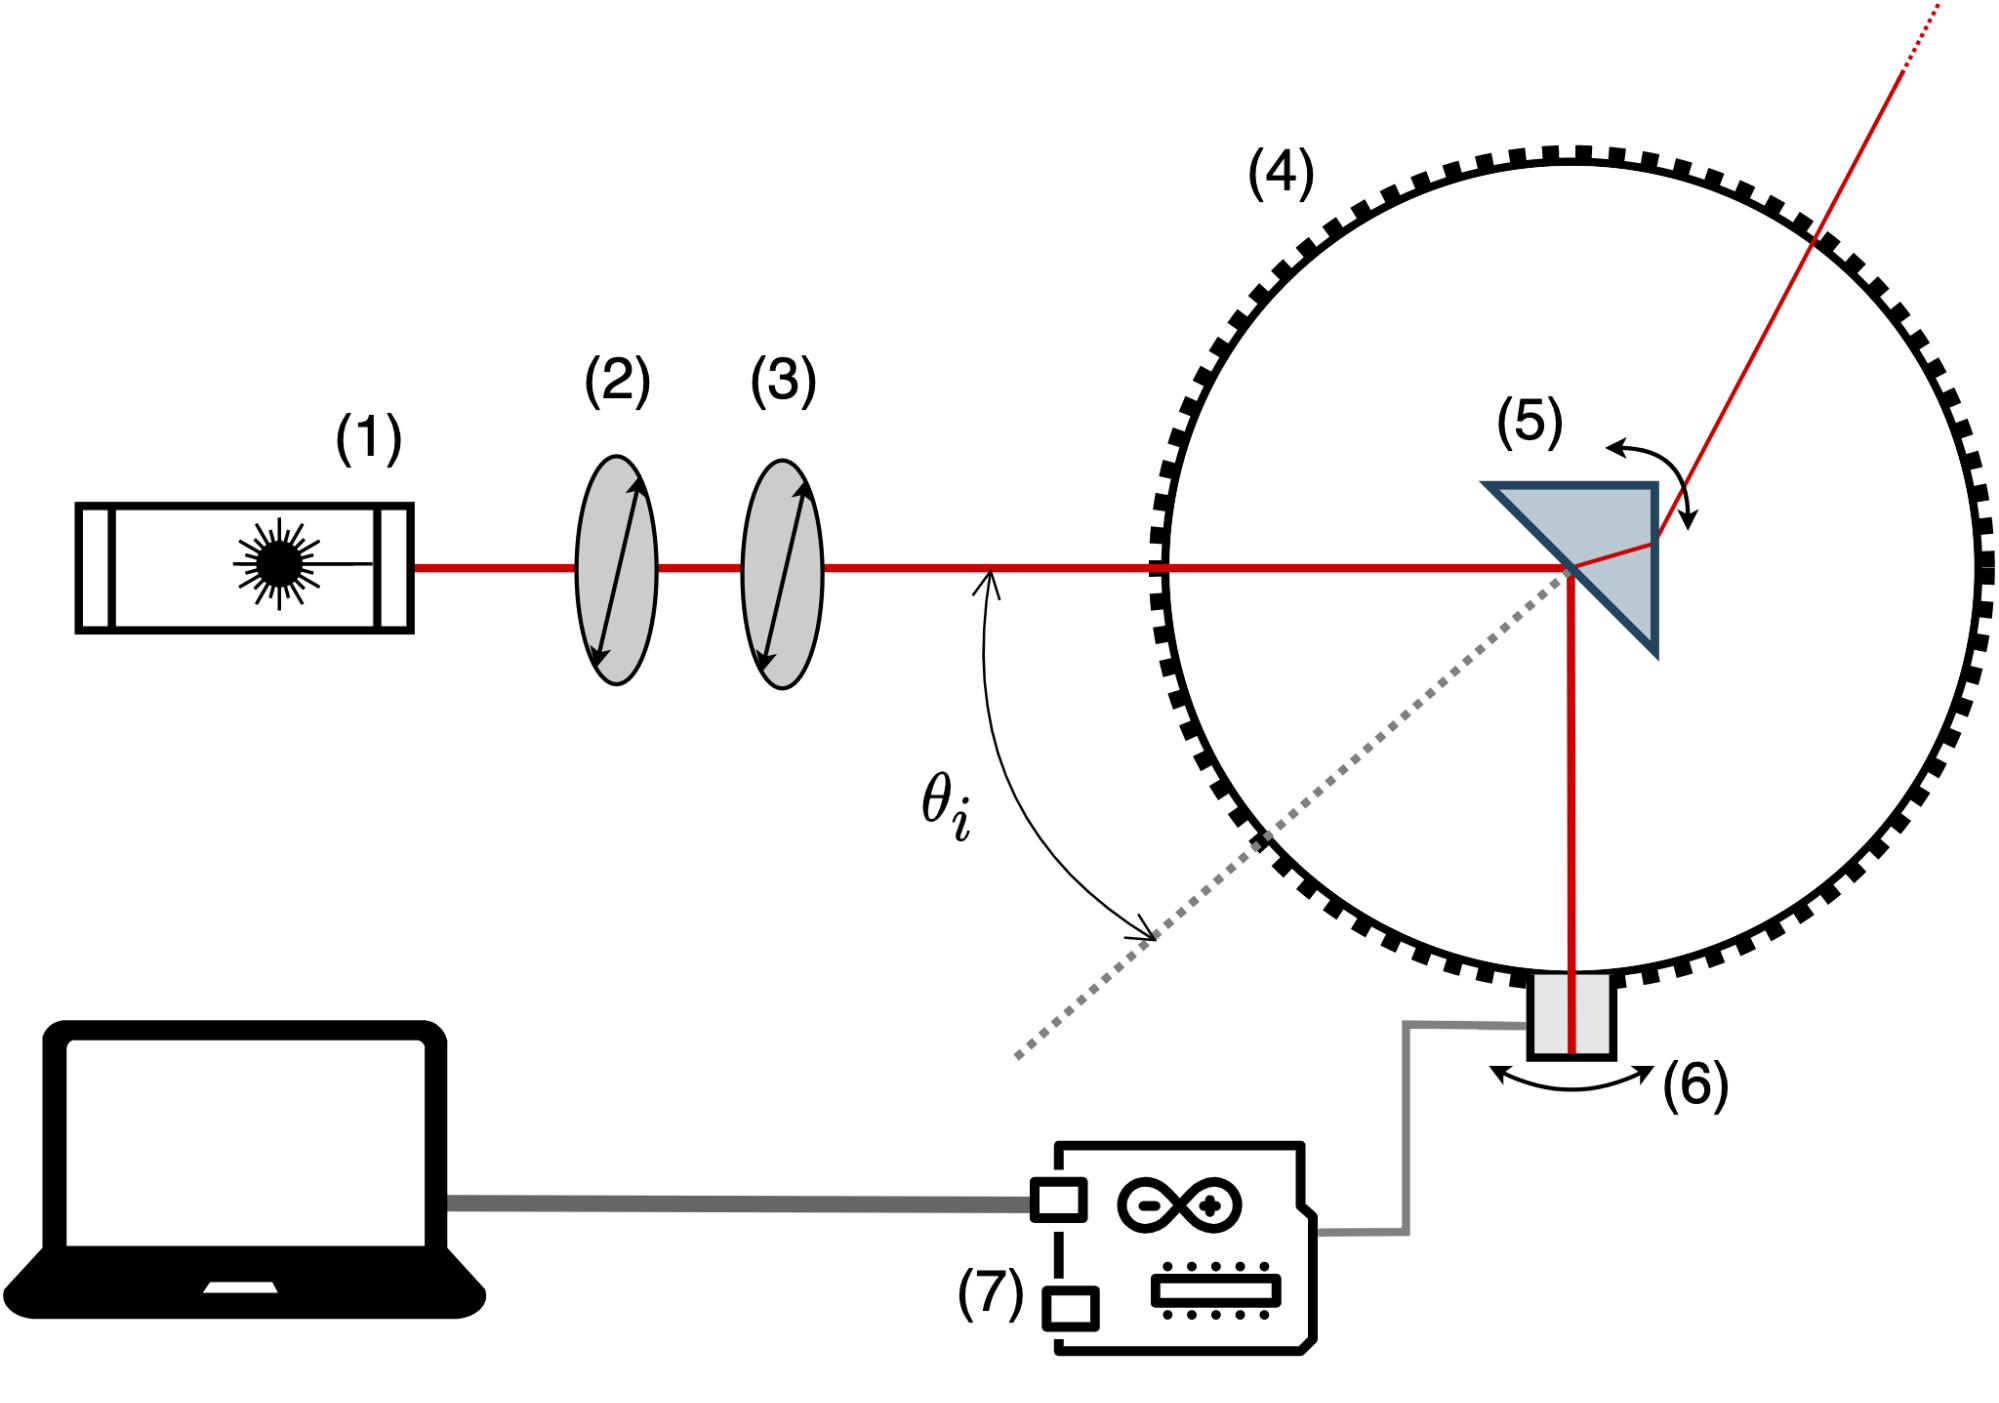
\includegraphics[width=8cm]{instrumental-apparatus.png}
      \caption{
        \emph{
          Apparato sperimentale. A partire da sinistra, in senso orario,
          si trovano: laser(a), filtri polaroid(b, c), guida circolare(d),
          prisma(e), sensore(f), Arduino(g). Il servomotore non è riportato.
        }
      }
      \label{fig:apparato-strumentale}
    \end{subfigure}%
    \hspace{5mm}
    \begin{subfigure}{.47\textwidth}
      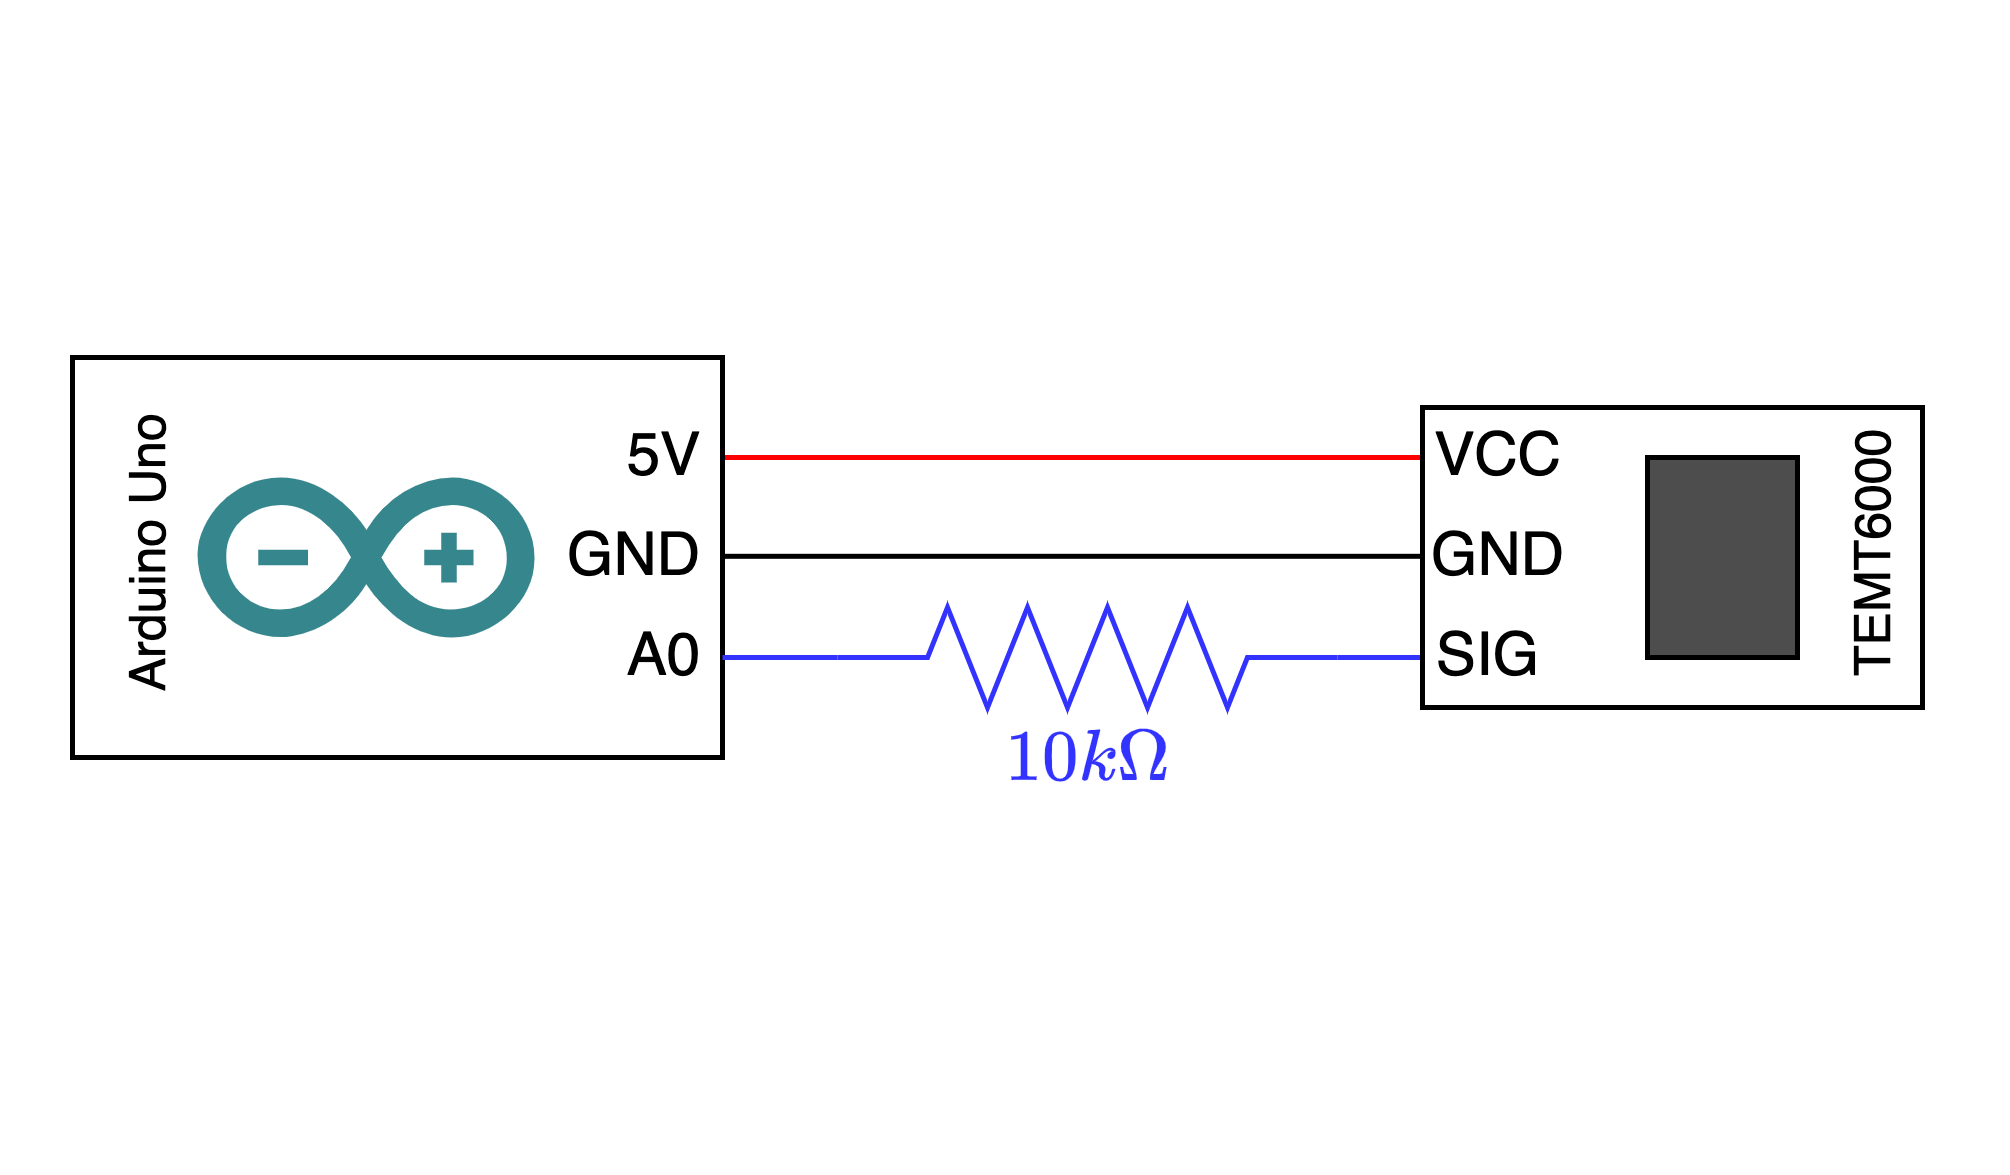
\includegraphics[width=8cm]{circuit-diagram.png}
      \caption{
        \emph{
          Schema circuitale. I pin $\text{VCC}$ e $\text{GND}$ del sensore sono collegati
          all'alimentazione di Arduino. Il pin $\text{SIG}$
          del sensore è collegato ad un input analogico di Arduino, tramite una
          resistenza da $10k\Omega$.
        }
      }
      \label{fig:diagramma-circuito}
    \end{subfigure}
    \caption{\emph{Apparato sperimentale e schema circuitale.}}
  \end{figure}
%
\subsection{Procedura sperimentale}\label{subsec:procedura-sperimentale}
  Abbiamo seguito la procedura sperimentale riportata di seguito, ripetuta due
  volte: una per raccogliere i dati relativi a $R_\pi$ e una per i dati relativi
  a $R_\sigma$. Questa procedura è stato adattata da quanto descritto in Lipson\cite{lipson20}.
  \begin{enumerate}
    \item%
      Abbiamo posizionato il polaroid(c) in modo che la polarizzazione del
      fascio laser fosse parallela al lato del prisma, e abbiamo aggiustato l'angolo
      del laser rispetto ad esso, in modo da evitare che il fascio
      polarizzato uscente dal laser venisse bloccato.
    \item%
      Abbiamo posizionato il sensore e il prisma in modo da rendere
      massimo l'angolo $\theta_i$, con il vincolo che
      tutto il fascio laser fosse contenuto sulla superficie del prisma\footnote{Per $\theta_i \to 90^\circ$, la
      proiezione del fascio laser sul prisma è un'ellisse di semiasse maggiore $a \to +\infty$. Chiaramente, non appena
      $a$ supera la lunghezza del lato del prisma, le equazioni \eqref{eq:fresnel-eq-p} e \eqref{eq:fresnel-eq-s} perdono
      la loro validità.}.
    \item%
      Ruotando il polaroid(b), abbiamo ridotto l’intensità del fascio laser
      incidente sul prisma, fino a che Arduino non ha potuto rilevare una
      variazione significativa del segnale del sensore.
      Questo ci ha permesso di sfruttare l'intero intervallo di operatività del convertitore analogico-digitale di Arduino.
    \item%
      Abbiamo acquisito l'intensità luminosa rilevata dal sensore in questo punto,
      poi abbiamo ruotato il prisma in senso orario e abbiamo
      allineato il sensore di conseguenza.
    \item%
      Abbiamo ripetuto il passo precedente fino a raggiungere un valore di $\theta_i$
      il più possibile vicino a zero.
    \item%
      Abbiamo ruotato di $90^\circ$ il polaroid(c) e ripetuto l'intera
      procedura un'altra volta.
  \end{enumerate}
  %
  I dati che abbiamo raccolto in questo modo \emph{non} sono
  i coefficienti $R_\pi$ e $R_\sigma$, ma differiscono da essi per una costante
  moltiplicativa $I_0$; questa verrà determinata tramite un \emph{fit}\footnote{Avremmo potuto misurare
  questo valore direttamente, ma così facendo avremmo dovuto
  abbassare ulteriormente l'intensità del fascio laser e non avremmo più potuto
  sfruttare l'intero intervallo di operatività di Arduino.}, come descritto in Sez.$\ref{subsec:analisi-coefficienti}$.
\endinput

